Using SI units, the given system data are
\[
L=0.568\ \mathrm{m},\quad m=5.35\ \mathrm{kg},\quad E=200\times10^{9}\ \mathrm{Pa},
\]
\[
b=0.037\ \mathrm{m},\quad h=0.003\ \mathrm{m},\quad u_0=0.0054\ \mathrm{m},
\quad v_0=0.
\]
These values use SI units throughout, so the displacement response will first be calculated in metres.

\[
\boxed{\begin{aligned}
L&=0.568\ \mathrm{m}, &m&=5.35\ \mathrm{kg}, &E&=200\ \mathrm{GPa},\\
b&=0.037\ \mathrm{m}, &h&=0.003\ \mathrm{m}, &u_0&=5.4\ \mathrm{mm},\quad v_0=0
\end{aligned}}
\qquad\text{(C.4.1)}
\]

For the rectangular flex-beam cross-section, the second moment of area about the bending axis is
\[
I=\frac{bh^3}{12}
 =\frac{(0.037)(0.003)^3}{12}
 =8.325\times10^{-11}\ \mathrm{m^4}.
\]
Because \(1\ \mathrm{m^4}=10^{12}\ \mathrm{mm^4}\), this is \(83.25\ \mathrm{mm^4}\).

\[
\boxed{I=8.325\times10^{-11}\ \mathrm{m^4}=83.25\ \mathrm{mm^4}}
\qquad\text{(C.4.2)}
\]

The flexural rigidity follows by multiplying the second moment of area by Young's modulus. Therefore,
\[
EI=(200\times10^9)(8.325\times10^{-11})=16.65\ \mathrm{N\,m^2}.
\]

\[
\boxed{EI=16.65\ \mathrm{N\,m^2}}
\qquad\text{(C.4.3)}
\]

A cantilever beam with a concentrated tip load has the end displacement \(\Delta=PL^3/(3EI)\). Hence its equivalent transverse stiffness is
\[
k=\frac{P}{\Delta}=\frac{3EI}{L^3}
 =\frac{3(16.65)}{(0.568)^3}
 =272.5778\ \mathrm{N/m}.
\]

\[
\boxed{k=272.58\ \mathrm{N/m}}
\qquad\text{(C.4.4)}
\]

With displacement measured from the undeformed reference used for this horizontal system, the undamped equation of motion is \(m\ddot u+ku=0\). Dividing by \(m\) gives \(\ddot u+\omega_n^2u=0\), where \(\omega_n^2=k/m\). Thus,
\[
\omega_n=\sqrt{\frac{k}{m}}
 =\sqrt{\frac{272.5778}{5.35}}
 =7.1379\ \mathrm{rad/s}.
\]

\[
\boxed{\omega_n=7.138\ \mathrm{rad/s}}
\qquad\text{(C.4.5)}
\]

The cyclic natural frequency is the angular natural frequency divided by \(2\pi\), so
\[
f_n=\frac{\omega_n}{2\pi}=\frac{7.1379}{2\pi}=1.1360\ \mathrm{Hz}.
\]

\[
\boxed{f_n=1.136\ \mathrm{Hz}}
\qquad\text{(C.4.6)}
\]

The period is the time for one complete oscillation. Therefore,
\[
\tau=\frac{1}{f_n}=\frac{2\pi}{\omega_n}=0.88026\ \mathrm{s}.
\]

\[
\boxed{\tau=0.8803\ \mathrm{s}}
\qquad\text{(C.4.7)}
\]

The general solution of the undamped equation is
\[
u(t)=A\cos(\omega_nt)+B\sin(\omega_nt).
\]
At \(t=0\), the initial displacement gives \(A=u_0\), while the initial velocity gives \(B=v_0/\omega_n\). Since \(v_0=0\), the response reduces to
\[
u(t)=u_0\cos(\omega_nt)=0.0054\cos(7.1379t)\ \mathrm{m}.
\]
Evaluating this expression at \(t_1=10\ \mathrm{s}\) gives
\[
u(10)=0.0054\cos\bigl(7.1379(10)\bigr)=-0.00344903\ \mathrm{m}=-3.44903\ \mathrm{mm}.
\]

\[
\boxed{u(10\ \mathrm{s})=-3.449\ \mathrm{mm}}
\qquad\text{(C.4.8)}
\]

For \(N_{\mathrm{osc}}=25\), the plotting interval ends at
\[
t_{\mathrm{end}}=N_{\mathrm{osc}}\tau=25(0.88026)=22.0065\ \mathrm{s}.
\]
The plotted response is shown below. The square marker identifies the calculated value at \(t_1=10\ \mathrm{s}\), and the same value can be read with a data tip.

\begin{figure}[H]
\centering
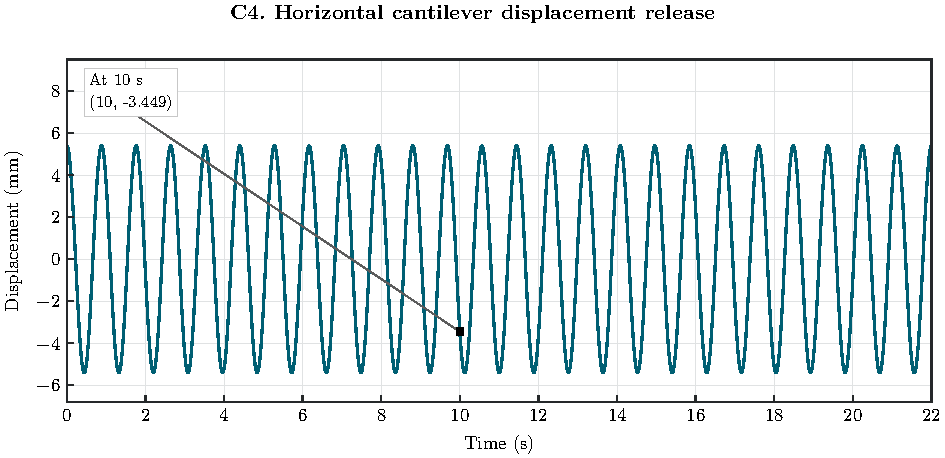
\includegraphics[width=0.95\linewidth,height=0.36\textheight,keepaspectratio,alt={C.4. Twenty-five oscillations with the ten-second response marked.}]{figures/generated/solutions/C4.pdf}
\caption{C.4. Twenty-five oscillations with the ten-second response marked.}
\end{figure}

\matlabcaption{C.4 response plot.}
\lstinputlisting[style=hwmatlab]{matlab/C4.m}

\[
\boxed{\begin{gathered}
t_{\mathrm{end}}=22.0065\ \mathrm{s}\quad\text{for}\quad N_{\mathrm{osc}}=25,\\
u_{\mathrm{tip}}(10\ \mathrm{s})=-3.449\ \mathrm{mm}
\end{gathered}}
\qquad\text{(C.4.9)}
\]

The computed displacement and the data-tip value agree because both use the same undamped response. The displacement changes sign as the mass passes through equilibrium, but its maximum absolute value remains \(u_0=5.4\ \mathrm{mm}\). Since no damping or external force is included, the oscillation continues with constant amplitude and period.

\[
\boxed{\max|u(t)|=5.4\ \mathrm{mm},\qquad \tau=0.8803\ \mathrm{s}\ \text{with constant amplitude}}
\qquad\text{(C.4.10)}
\]
